\documentclass[a4paper]{article}

\usepackage{pgfplots}

\begin{document}

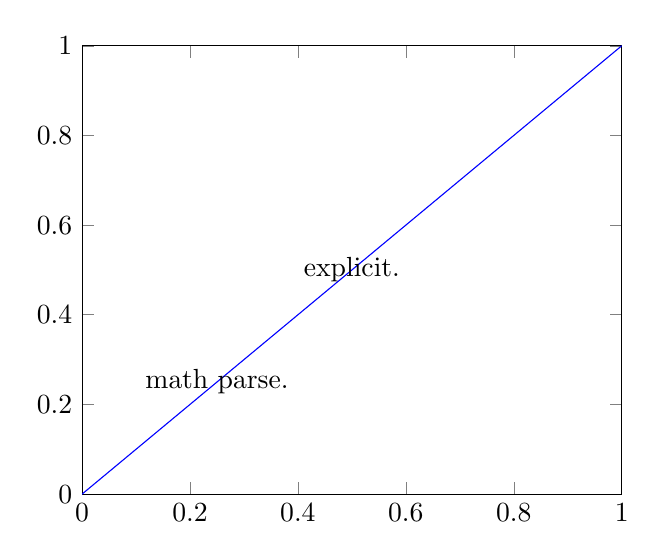
\begin{tikzpicture}
%\tracingcommands=2\tracingmacros=2
	\begin{axis}[xmin=0,xmax=1,ymin=0,ymax=1]
	\addplot+[mark=none,samples=2] {x};

	\node at (axis cs:0.5,0.5) {explicit.};

	\node at (axis cs:1/4,1/4) {math parse.};
	\end{axis}
\end{tikzpicture}

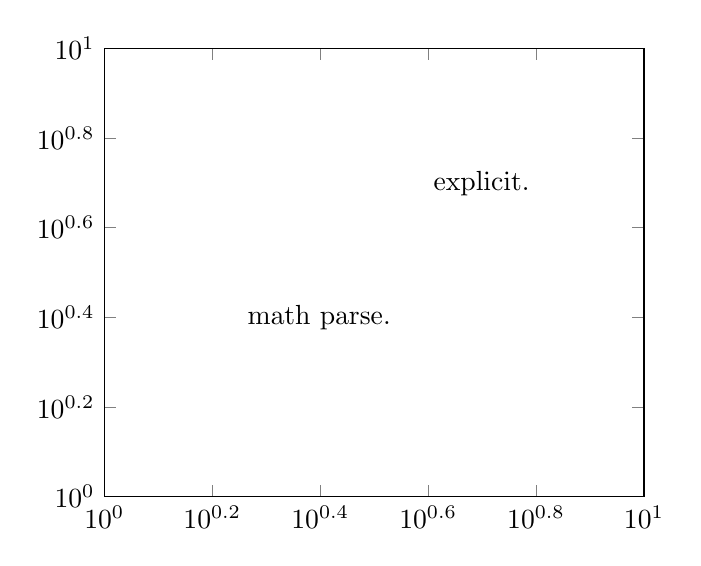
\begin{tikzpicture}
%\tracingcommands=2\tracingmacros=2
	\begin{loglogaxis}[xmin=1e0,xmax=1e1,ymin=1e0,ymax=1e1]
	\addplot+[domain=1e-5:5,mark=none,samples=2] {exp(x)};

	\node at (axis cs:5,5) {explicit.};

	\node at (axis cs:1e1/4,1e1/4) {math parse.};
	\end{loglogaxis}
\end{tikzpicture}
\end{document}

